\begin{figure}[p]
\centering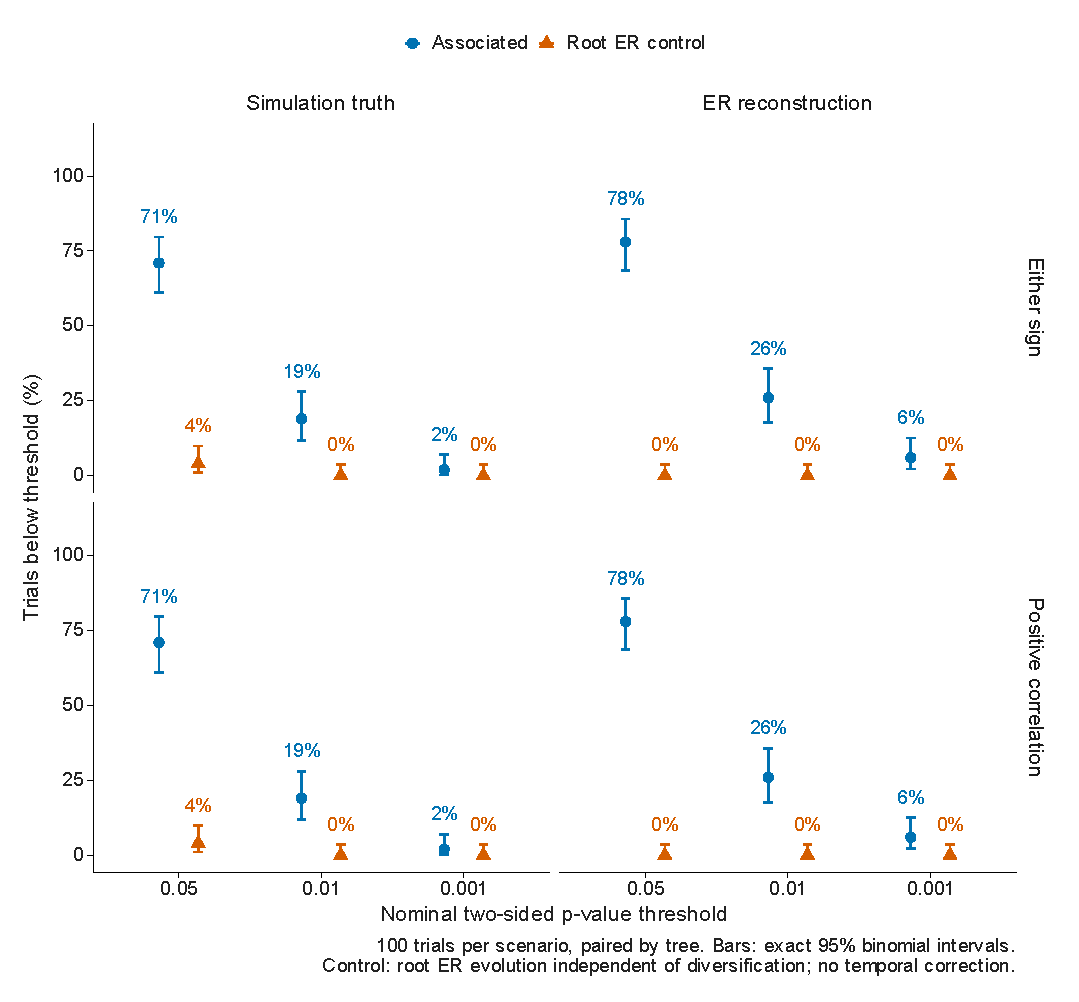
\includegraphics[width=\textwidth]{../figures/scenario-p-value-percentages.pdf}
\caption{Nominal detection under associated and independent-character scenarios.
Each scenario contains 100 trials paired by tree. The upper row includes
correlations of either sign; the lower row requires a positive correlation.
Columns distinguish exact simulated histories from reconstructed histories.
Bars are exact 95\% binomial intervals. Control frequencies quantify false
association under homogeneous root ER, with the same tree conditioning and
uncorrected temporal Pearson tests as the associated scenario.}
\label{fig:paired-detection}
\end{figure}
\begin{figure}[p]
\centering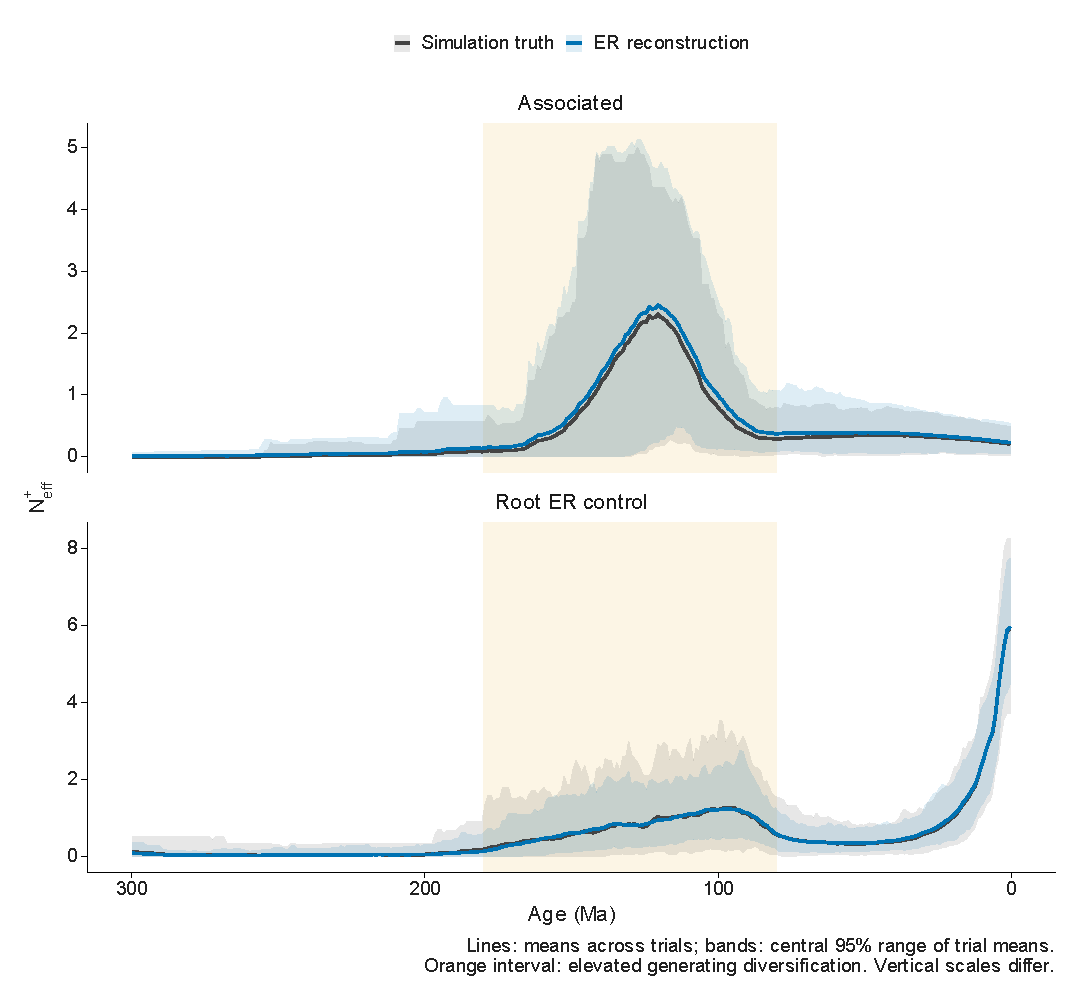
\includegraphics[width=\textwidth]{../figures/scenario-neff-through-time.pdf}
\caption{Mean diversity trajectories in the paired scenarios. Bands show the
central 95\% range of trial means, not uncertainty in the grand mean.
Orange shading marks elevated generating diversification. Vertical scales
differ. The homogeneous transition rate in the control does not imply that
a realized branch-based diversity statistic must be constant through time.}
\label{fig:paired-curves}
\end{figure}
\begin{figure}[p]
\centering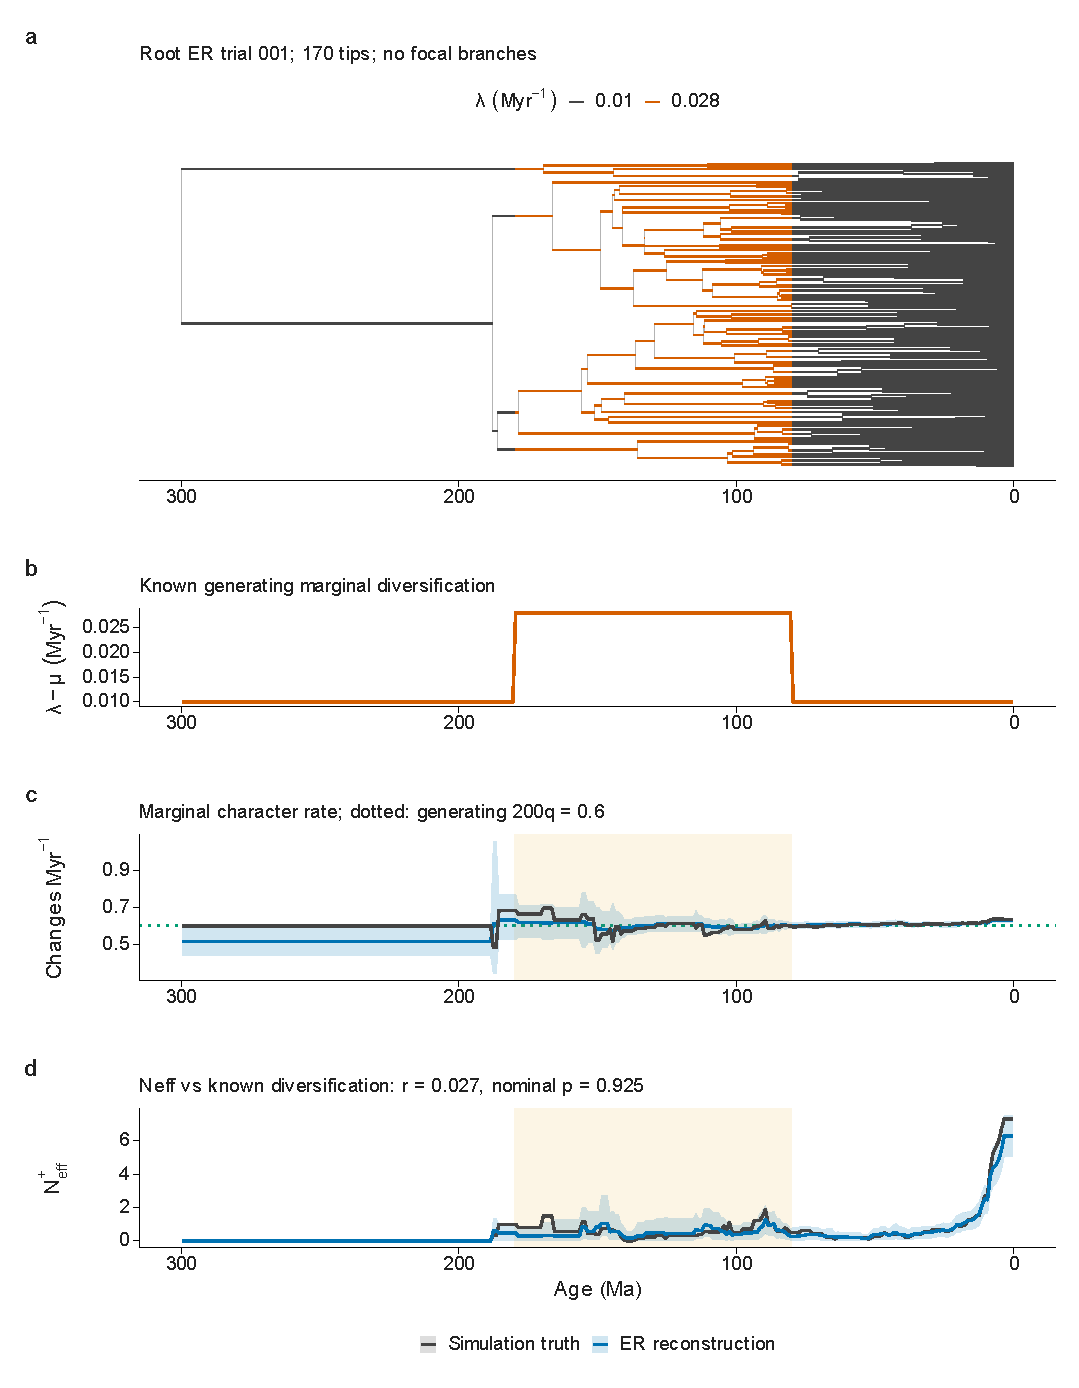
\includegraphics[width=0.93\textwidth]{../figures/trial-001-overview.pdf}
\caption{Prespecified control trial 001. The tree is coloured by the known
generating speciation rate. Diversification is taken directly from the
generator, whereas reconstructed marginal character rates and diversity use
ER fits and conditional stochastic maps of terminal observations. Grey
curves use actual simulated histories. The dotted green line is the constant
expected generating character rate, $200q=0.6$ changes per lineage per Myr.
Bands are central 95\% intervals
across maps, conditional on fitted parameters. All 100 control trials are
shown in the accompanying diagnostic atlas.}
\label{fig:null-example}
\end{figure}
\begin{figure}[p]
\centering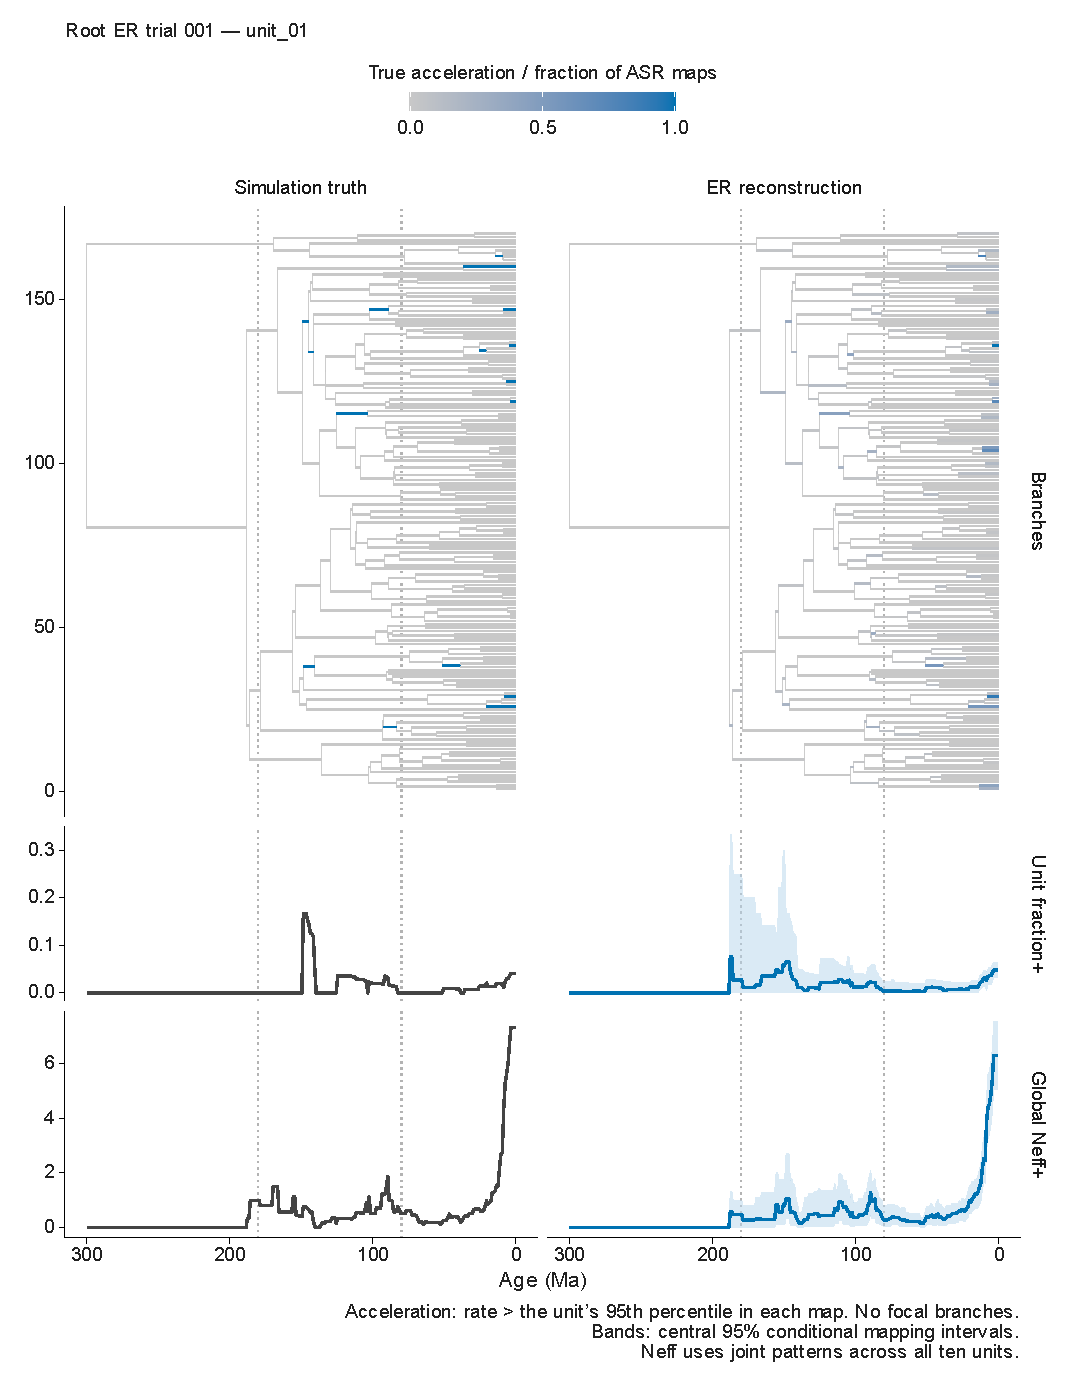
\includegraphics[page=1,width=0.93\textwidth]{../figures/trial-001-unit-acceleration.pdf}
\caption{Unit 01 in control trial 001. The upper panels show actual branch
acceleration and the proportion of reconstructed maps classifying each
branch as accelerated. The middle panels show the fraction of active
lineages accelerated for this unit; the lower panels show global
$N_{\mathrm{eff}}^{+}$ from joint patterns across all ten units. Vertical
lines mark the diversification epoch boundaries. There are no focal
branches in this control. The complete ten-unit atlas is supplied separately.}
\label{fig:null-unit}
\end{figure}
